\documentclass[12pt,fleqn]{article}\usepackage{../../common}
\begin{document}
Green'in Teorisi, Uzaklaşım, Stokes

Green'in Teorisi

Bu teorinin detayları, ispatı [2]'de bulunabilir. Tekrar üzerinden geçmek
gerekirse, [4, sf. 429] bazlı anlatalım, iki boyutta elimizde bir $D$ bölgesi
etrafındaki $C$ eğrisi var, ve $F(x,y) = M(x,y) \textbf{i} + N(x,y) \textbf{j}$
$D$ içinde vektör alanı olsun, o zaman alttaki ifade doğrudur,

$$
\int_C M \ud x + N \ud Y =
\int \int_D \left(
  \frac{\partial N}{\partial x} - \frac{\partial M}{\partial y}
  \ud x \ud y
\right)
$$

$\int_C$ ki bazen $\oint_C$ ile gösterilir, bir eğri üzerinden alınan bir
entegraldır. Eşitliğin sol tarafı bazen bir $\ud\vec{s}$ üzerinden de
sunulabilir,

$$
\int_C \vec{F} \cdot \ud\vec{s} = \int_C M \ud x + N \ud Y 
$$

Bu cebirsel bir özet sadece, $\ud{\vec{s}} = [\begin{array}{cc} \ud x & \ud y \end{array}]^T$
sonuçta ve noktasal çarpım bize iki üstteki ifadeyi verecektir.

olarak ta gösterilebilir.

Örnek

Bir vektör alanı $\vec{F} = xy \textbf{i} + y^2 \textbf{j}$ olsun, ve bu alanda
birinci dörtlük içinde $y = x$ çizgisi ve $y=x^2$ parabölü arasındaki bölgeyi
düşünelim. Bu bölge ve alan üzerinden Green'in Teorisini doğrulamaya uğraşalım.

Grafik şu şekilde,

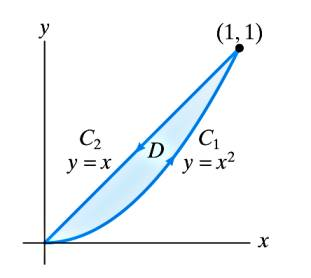
\includegraphics[width=15em]{calc_multi_75_green_02.jpg}

Vektör alanı (100 ile çarpıp vektörleri büyüttük gözüksün diye),

\begin{minted}[fontsize=\footnotesize]{python}
x = np.linspace(0,1.,10)
y = np.linspace(0,1.,10)
x,y = np.meshgrid(x,y)
SCALE = 100.0
u = x*y*SCALE; v = (y**2)*SCALE
v = np.zeros(y.shape)
q = plt.quiver(x,y,u,v,angles='xy',scale=1000,color='r')
p = plt.quiverkey(q,1,16.5,50,"50 m/s",coordinates='data',color='r')
plt.savefig('calc_multi_75_green_01.jpg')
\end{minted}

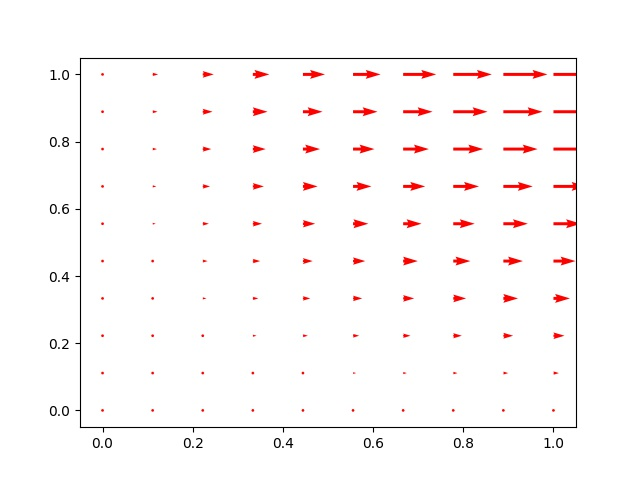
\includegraphics[width=15em]{calc_multi_75_green_01.jpg}

Eğri iki parça olarak analiz edilecek, $C_1$ ve $C_2$.  Eğri üzerinden gereken
tüm entegral,

$$
\int_C \vec{F} \cdot \ud{\vec{s}} = \int_C xy \ud x + y^2 \ud y
$$

Bu entegral iki parça üzerinden alınmalı ve sonuç toplanmalı,

$$
= \int_{C_1} xy \ud x + y^2 \ud y + \int_{C_2} xy \ud x + y^2 \ud y
\label{2}
$$

Eğriyi parametrize edelim, böylece $\ud x$, $\ud y$ üzerinden entegraller
kolaylaşsın,

$$
C_1: x = t, y = t^2, \quad 0 \le t \le 1
$$

$$
C_2: x = 1-t, y = 1-t, \quad 0 \le t \le 1
$$

$C_1$,$C_2$ gidişat yönlerine dikkat, mesela eğri ile yukarı çıkış var, ama düz
eğri ile aşağı ınıyoruz, bu sebeple $t$ sıfırdan başlarken $x,y$ değerleri
$(1,1)$, öyle ayarladık, ve en sonda $t=1$ olduğu anda $x,y$ değerleri $(0,0)$
oluyor. 

Şimdi parametrize edilmiş değişkenlerle (2) formülünü tekrar yazalım,

$$
= \int_{0}^{1} ( t \cdot t^2 + t^4 \cdot 2t ) \ud t +
\int_{0}^{1} ((1-t)^2 + (1-t)^2) (-\ud t)
$$

$$
= \int_{0}^{1} (t^3 + 2t^5) \ud t + \int _{0}^{1} 2 (1-t)^2 (-\ud t)
$$

$$
= (\frac{1}{4} t^4 + \frac{2}{6} t^6) \big\vert_{0}^{1} +
(\frac{2}{3} (1-t)^3 ) \big\vert_{0}^{1}
$$

$$
= \frac{1}{4} + \frac{2}{6} - \frac{2}{3} = -\frac{1}{12}
$$

[devam edecek]

Gauss-Green Eşitliği

Gauss-Green eşitliği iki boyutta şu şekilde gösterilebilir [1, sf. 262],

$$
\iint_R (\nabla u ) \cdot w \ud x \ud y =
\iint_R u (- \bdiv w) \ud x \ud y + \int_C u w \cdot n \ud s
$$

Türetmek için başlangıç noktası $uv$ üzerinde uzaklaşım almak. Aslında
ileride göreceğimiz gibi çok boyutta parçalı entegral tekniği Gauss-Green'in
uzantısı bir bakıma ve tek boyutta gördük ki [3] parçalı entegrale erişmek
için de Calculus'un çarpım kuralından başlanmıştı.

$$
\bdiv (uw) = \bdiv (u w_1 + u w_2) =
\frac{\partial u}{\partial x} w_1 +
\frac{\partial w_1}{\partial x} u +
\frac{\partial u}{\partial y} w_2 +
\frac{\partial w_2}{\partial y} u 
$$

Gruplarsak,

$$
= \left( 
\frac{\partial u}{\partial x} w_1 +
\frac{\partial u}{\partial y} w_2 \right) +
\left( 
\frac{\partial w_1}{\partial x} u +
\frac{\partial w_2}{\partial y} u \right)
$$

Daha kısa şekilde,

$$
\bdiv (uw) = \nabla u \cdot w + u \bdiv(w)
$$

Üstteki ifade üzerinde Uzaklaşım Teorisi'ni uygulayalım. Önce
$\iint_R \bdiv (uw)$,

$$
\iint_R \bdiv (uw) \ud x \ud y= \iint_R \nabla u \cdot w + u \bdiv(w) \ud x \ud y
$$

$$
= \iint_R \nabla u \cdot w  \ud x \ud y + \iint_R u \bdiv(w) \ud x \ud y
$$

Uzaklaşım Teorisi'ne göre sağ taraf $\int_C uw \cdot n \ud s$ olmalı, yani

$$
\iint_R \nabla u \cdot w  \ud x \ud y + \iint_R u \bdiv(w) \ud x \ud y = \int_C uw \cdot n \ud s
$$

Eşitliğin sol tarafındaki ikinci terimi sağa geçirirsek,

$$
\iint_R \nabla u \cdot w  \ud x \ud y =
\iint_R u (-\bdiv w) \ud x \ud y + \int_C uw \cdot n \ud s
$$

[1] notasyonu ile $\nabla$ yerine $\grad$,

$$
\iint_R \grad u \cdot w  \ud x \ud y =
\iint_R u (-\bdiv w) \ud x \ud y + \int_C uw \cdot n \ud s
\mlabel{3}
$$

Böylece Gauss-Green eşitliğine erişmiş olduk.

Green'in İlk Eşitliği 

Eğer (3) içinde $w$ için $\grad u$ sokarsak, bu bize Green'in İlk Eşitliği (Green's First
İdentity) denen formülü veriyor [1, sf. 281], 

$$
\iint_R \grad u \cdot \grad u  \ud x \ud y =
\iint_R u (-\bdiv \grad u) \ud x \ud y + \int_C u \grad u \cdot n \ud s
$$

Gradyanın uzaklaşımı bazen $\Delta$ notasyonu ile gösterilir, öyle yapalım,

$$
\iint_R | \grad u |^2  \ud x \ud y = - \iint_R u (\Delta u) \ud x \ud y +
\int_C u \grad u \cdot n \ud s
$$

Eşitliğin sağından, solundan birkaç yer değişim sonrası,

$$
\iint_R u (\Delta u) \ud x \ud y =
- \iint_R | \grad u |^2  \ud x \ud y
+ \int_C u \grad u \cdot n \ud s
$$

Böylece [1, sf. 281]'daki forma erişmiş olduk. Bu Green'in İlk Eşitliği.

[devam edecek]

Kaynaklar

[1] Strang, {\em Computational Science and Engineering}

[2] Bayramli, {\em Cok Degiskenli Calculus, Ders 23}

[3] Bayramlı, {\em Diferansiyel Denklemler, Ekler}

[4] Colley, {\em Vector Calculus}

\end{document}
